% Document template based on LNCS, adapted by Matt Welsh <mdw@cs.berkeley.edu>

% This version is adapted to use PDFTEX to render to PDF directly. 
% If you want to use dvi, you need to change any figures to use '.eps'
% rather than '.pdf', and probably get rid of the hyperref package.

\documentclass{article}
\usepackage{program}
\usepackage{acm-style10} % ACM proceedings formatting
\usepackage{times}       % Use Adobe Times font set
\usepackage{epsfig,twocolumn}
\usepackage{url}
\usepackage[english]{babel} % mdw: Required to get good hyphenation on RH6.0
                            % (fixed in RH6.1)
\usepackage{subfigure}
\usepackage{graphicx} 
\usepackage{color}

% DO NOT EDIT THE BELOW BLOCK OF CODE
\def\dsp{\def\baselinestretch{1.10}}
\dsp
\newcommand{\XXXnote}[1]{{\bf\color{red} XXX: #1}}
\setlength{\textheight}{9.25in}
\setlength{\columnsep}{0.33in}
\setlength{\textwidth}{7.4in}
\setlength{\footskip}{0.0in}
\setlength{\topmargin}{-0.25in}
\setlength{\headheight}{0.0in}
\setlength{\headsep}{0.0in}
\setlength{\oddsidemargin}{-.45in}
\setlength{\parindent}{1pc}
\pagestyle{empty}
\begin{document}
\date{}

%%%%%%%%%%%% THIS IS WHERE WE PUT IN THE TITLE AND AUTHORS %%%%%%%%%%%%

% Title here
\title{\ttlfnt Compression for Wireless Sensor Networks}

% Author names, affiliations, and e-mail below
\author{{\aufnt Daniel Shteremberg} \\ 
{\affaddr Harvard University}\\ 
{\affaddr dshterem@fas.harvard.edu}
\and {\aufnt Jason Waterman} \\
{\affaddr Harvard University}\\ 
{\affaddr waterman@eecs.harvard.edu}
}

\maketitle
%\copyrightspace
\thispagestyle{empty}

%%%%%%%%%%%%%  ABSTRACT GOES HERE %%%%%%%%%%%%%%

\subsection*{Abstract}
\begin{small}
Abstract
\end{small}

%%%%%%%%%%%%%  BODY OF PAPER GOES HERE %%%%%%%%%%%%%%

% Generally you will want to break the paper into separate sections
% and use \input{...} to include them, like so:
\section{Introduction} 

Wireless sensor networks involve collections of many battery operated
nodes that can number in the thousands.  A canonical example of a
sensor node is the Telos Mote~\cite{telos} (colloquially referred to
as a mote) which has a 16-bit microcontroller running up to 8 MHz, 48
KB of program memory, 10 KB of ram, and a 2.4 GHz 802.15.4 radio with
an effective data rate of 250 kbps.  This is five orders of magnitude
difference in memory size, four orders of magnitude of difference in
networking speed, and three orders of magnitude difference in
processing speed than a typical desktop computer or laptop.  These
sensor networks are often powered by only a pair AA batteries and are
expected to last months or even years on such a limited power source.

As implied in their name, the primary goal of a sensor networks is to
sense and report on their surrounding habitat. As the field has
matured from some of the early low data-rate habitat monitoring
applications such as Great Duck Island~\cite{gdi-sensys04}, a new
class of sensor network applications have emerged requiring high data
rates, high data fidelity requirements, and computationally intensive
processing. Examples of applications in this class include vibration
monitoring of bridges and
buildings~\cite{brimon,netshm-spots06,ggb-monitoring}; seismic
monitoring of fault zones and
volcanoes~\cite{ucla-seismic,volcano-osdi06}; acoustic monitoring of
animal habitats~\cite{girod-marmots,enviromic}; and body sensor
networks for monitoring activity and
movement~\cite{intel-msp,satire,parkinsons-embs07}.  These
applications present several unique challenges to sensor networks.
The amount of data being generated by these systems outstrips the
radio's ability to transmit this data (say to a base station).
Compression is one way to help cope with the volume of data that these
applications produce.  

Due to limited energy available to these systems, reducing power is of
primary importance.  Of the energy costs, radio transmissions and
receptions dominate the energy budget.  The radio, both in
transmission and reception, uses an order of magnitude more power than
just processing alone~\cite{telos}.  Because of the high energy costs
to send and receive data, there can be a large potential energy
savings if the sensor nodes are able to compress their data before
transmitting.

Because most sensor networks are spatially many times larger than
their radio range, sensor networks often use multi-hop routing to move
data across the network.  Because of multi-hop routing, compression
not only obtains a savings of energy at the node level, but also at
any node that this data passes through on its way to its destination.

But most sensor networks do not use data compression.  The problem is
that because of the limited processing power and the extremely
constrained memory on these devices, implementing traditional
compressions schemes are non-trivial.  For example, many compression
schemes, like LZ77~\cite{lz77}, use large data buffers in the
compression algorithm.  Sensor network nodes, with their extremely
limited memory budget will not be able to have such a large window,
and compression ratios will suffer.

In this paper we look at three data sources: seismic volcano data,
acoustic wildlife data, and motion data collected from a body sensor
nework which were collected from actual sensor network deployments.
We find that traditional compression schemes such as LZ77 and Huffman
Encoding, in addition to being difficult to implement on resource
constrained nodes, did not provide very good compression rations.  




 
\section{Related Work}

\section{LZ77}

LZ77 \cite{lz77} seemed like a promising algorithm for Wireless Sensor
Network compression. Unlike LZW \cite{lzw} and other dictionary
building schemes, LZ77 maintains a constant size back-buffer with
which it performs matches. Without an upper bound on the dictionary
size, it is unreasonable to use dictionary based compression
algorithms because it is very easy to run out of memory on sensor
motes. LZ77, on the other hand, requires a constant amount of memory,
and using a pointer based circular buffer, it would be easy to
implement LZ77 on a mote without having to copy large pieces of
memory.

However, in practice, LZ77 does not perform as well. Further
investigation of LZ77 implementations revealed that these
implementations use large back-buffers, sometimes as big as 64k
entries. Many times, pure LZ77 is not implemented, but a history
dictionary is built in order to find matches more quickly. This
growing dictionary makes LZ77 prohibitive on sensor motes. Without a
history dictionary, matches can take a long time because the entire
back buffer must be searched for each new element that comes in. In
order to quantify how well LZ77 performs on our three data sets, we
compressed our data using a standard implementation of LZ77.

\begin{table}
  \begin{center}
  \begin{tabular}{|l||r|r|r|}
    \hline
    & LZ77 & RLE & Huffman \\ \hline
    Volcano & 99.7\% & 100.1\% & 81.6\% \\ \hline
    SHIMMER & 88.5\% - 98.8\% & 100.1\% & 70.8\% \\ \hline
    Marmot chirps & 98.5\% & 100.2\% & 70.2\% \\ \hline
    
  \end{tabular}
  \end{center}
  \caption{Compression ratios using standard methods}
  \label{table:compratios}
\end{table}

Table~\ref{table:compratios} shows the compression ratios for our
three data sets; high ratios mean bad compression. Note that LZ77
performs very poorly as the best compression ratio is 88.5\%. We used
a back-buffer size of 1024, which is a reasonable size for a mote
implementation. LZ77 performs so poorly for several reasons. First,
the back-buffer is not large enough to find a large amount of
matches. Also, the noise in the data makes matching very difficult. We
are not compressing english text, where there is no noise, instead we
are compressing sensor readings coming from an ADC, which have an
inherent amount of noise.

Table~\ref{table:compratios} also shows the compression ratios of two
other schemes: Run Length Encoding (RLE) and Huffman encoding. RLE
works by encoding consecutive duplicates with two numbers: the
element, and the length of the run. Due to the noise in our data,
there are very few runs, which is why RLE does so poorly. Huffman
coding does somewhat better, but it requires building a tree of prefix
codes. This tree could be very large, depending on how many bits each
sample has. For this reason, Huffman coding is not useful in a sensor
network context. 

These experiments have clearly shown that traditional techniques that
work in traditional computing environments, are not always suitable in
a sensor network context. We have not exhaustively tested all
compression schemes, but we have tested a few that are commonly
used. Moreover, complex algorithms are more difficult to implement on
sensor motes due to their limited debugging capabilities and lack of
mature development tools. We realize that the best compression scheme
for Wireless Sensor Networks is one that requires little computation,
is not very complex, and of course, has good compression ratios for
the sensor data.

\section{Variable Block Size Delta Encoding}

Given the inadequacies of standard compression schemes in the sensor
network context we developed a compression scheme that performs well
with sensor data, has minimal computation and is easy to implement on
motes. We decided to exploit the correlation between consecutive
samples. In sensor data, a sample is very likely to be close to the
previous sample. This characteristic lends itself nicely to delta
encoding. Because compression is very tied to data transmission in
sensor networks, our compression scheme must be designed for radio
transmission as well as the data we are compression. Whereas data
payload sizes in 802.11 packets are usually around 1500 bytes, data
payloads in 802.15.4 packets, which is the protocol used by sensor
motes, is between 30-100 bytes.

Given these requirements, we developed a variable block size delta
encoding scheme. For clarity of explanation, we will assume we are
working with 12 bit data and 30 byte packets. These characteristics
are those of the SHIMMER platform from which we obtained the
accelerometer data. However, this scheme works for higher order data
and larger packet sizes. All packets are fixed size, so we want to pack
as much information into a packet as possible. In addition, we want to
build some redundancy into the scheme. It might be possible to lose a
packet in sensor networks. However, since we are using delta encoding,
if we miss a packet, we still want to be able to decode the rest of
the data.

Each packet contains a block of data. Each block has a header and a
delta payload. The first sample in the block is stored in the header
uncompressed. This is for robustness so that if a packet is lost, only
the data in that packet is lost and not any subsequent data. The delta
is computed for every sample after the first with its previous
sample. The number of bits required to encode the delta is calculated
and stored. All of the deltas in the delta payload are encoded using
the same number of bits. The number of bits to encode the deltas is
therefore the number of bits needed to encode the largest delta. As
each sample comes in, the size of the block is calculated. If the
block still fits in the packet, the delta is added to the block. If
the block would not fit in the packet, the block is encoded into the
packet and dispatched. In the header we store the uncompressed first
element (12 bits), the block size (8 bits), and bits per delta (4
bits). The entire header fits into 3 bytes, leaving 27 bytes for the
delta payload. There are two reasons why a new sample would not fit in
the block. First, if the block already has many samples, a new delta
might simply not fit in the block. Secondly, if a very large delta
comes in, it would require that all the other deltas be encoded with
many more bits, which would push the entire block over the packet size
limit. 

This compression scheme is extremely simple to implement and requires
very little computation. For each sample, a delta must be calculated,
and it must be compared with the largest delta. When transmitting the
block, the deltas must be packed into the payload. Compared to LZ77 or
Huffman coding, this is very little computation. In the following
section we will evaluate this compression scheme using our data sets
and determine how well it performs. We will also quantify the effect
of noise on our scheme.


\section{Experiments and Results}

\begin{table}
  \begin{center}
  \begin{tabular}{|l||r|}
    \hline
    & VBS Delta Encoding \\ \hline
    Volcano & 53.3\% \\ \hline
    SHIMMER & 42.2\% - 62.8\% \\ \hline
    Marmot chirps & 33.1\% \\ \hline
    
  \end{tabular}
  \end{center}
  \caption{Compression ratios using Variable Block Size Delta Encoding}
  \label{table:vbsde}
\end{table}

We compressed our three data sets using our VBS Delta Encoding
scheme. These results are presented in Table~\ref{table:vbsde}. Notice
that the marmot chirp data set has the best compression ratio. This is
mostly due to a lower noise floor than the other data sets. In
addition, there is very little variablility in the data when there are
no chirps, and the occasional chirp has a short duration. Volcano data
has more noise and more frequent events. The SHIMMER data also has
noise, but it records constant movement, so there are longer duration
events with higher frequencies. However, these results show that our
delta encoding scheme outperforms LZ77, RLE, and Huffman encoding.

\subsubsection{Noise}

We performed a simple experiment to quantify how well our compression
scheme performs in the presence of noise. We took a constant data set
with a value of 3000 and added random gaussian noise. We varied the
standard deviation of the noise from 0 to
100. Figure~\ref{fig:noiseset} show a plot of four of these noise
intensities. Figure~\ref{fig:noiseall} shows the compression ratio as
a function of the noise standard deviation. When there is no noise the
compression ratio is 9.22\%. This is the lower bound compression ratio
for our scheme. Under perfect conditions (no noise and constant data),
our scheme is capable of achieving this compression ratio. The maximum
compression ratio with 100 standard devation noise is 69.08\%. From
Figure~\ref{fig:noiseall} we can see that adding a little noise has a
significant effect on the performances. However, after a certain
point, our scheme is robust to noise. A standard deviation of 100 for
12 bit data is quite high, and we don't expect data sets to have
anywhere near as much noise. For example, the marmot chirp data could
not have noise of any more than 4 standard deviation, otherwise it
would not have been compressed to 33.1\%.

\begin{figure*}[ht]
\centering
\subfigure {
  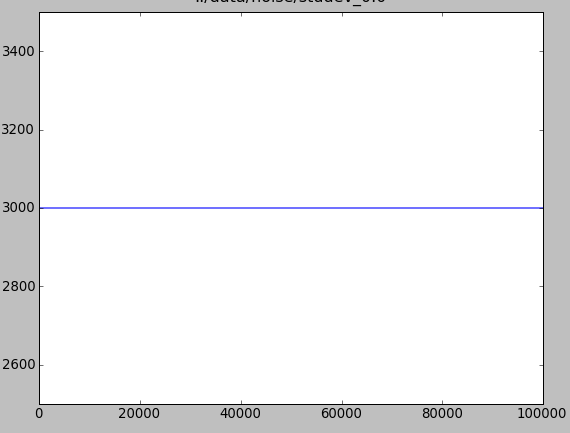
\includegraphics[width=0.22\textwidth]{figures/noise0.png}
  \label{fig:noise0}
}
\hfill
\subfigure {
  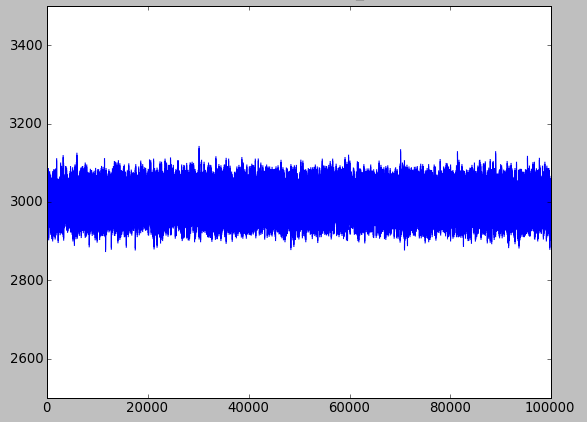
\includegraphics[width=0.22\textwidth]{figures/noise30.png}
  \label{fig:noise30}
}
\hfill
\subfigure {
  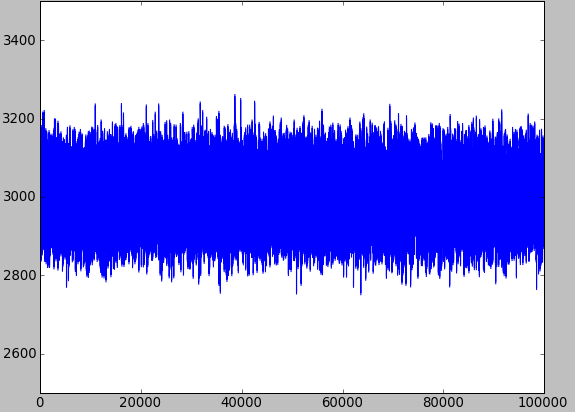
\includegraphics[width=0.22\textwidth]{figures/noise60.png}
  \label{fig:noise60}
}
\hfill
\subfigure {
  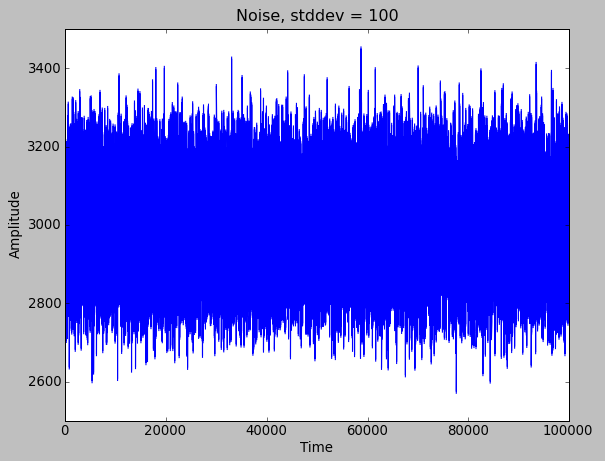
\includegraphics[width=0.22\textwidth]{figures/noise100.png}
  \label{fig:noise100}
}
\caption{Noise data set with standard deviation of 0, 30, 60 and 100}
\label{fig:noiseset}
\end{figure*}  

\begin{figure}
  \centering
  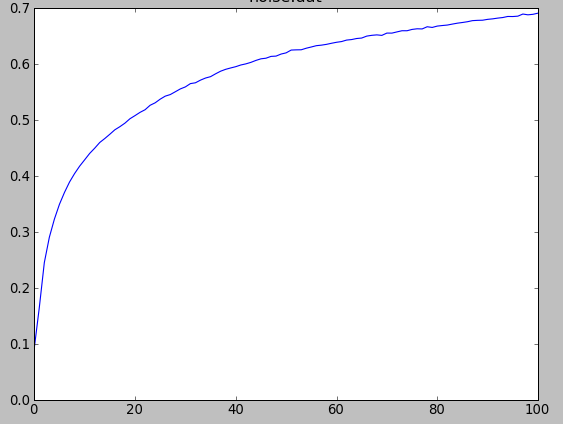
\includegraphics[width=0.50\textwidth]{figures/noiseall.png} 
  \caption{Compression ratio vs. standard deviation of noise}
  \label{fig:noiseall}
\end{figure}

\subsubsection{Energy}

\section{Future Work}

\section{Conclusion}


%%%%%%%%%%%%%  THIS IS WHERE THE BIBLIOGRAPHY GOES %%%%%%%%%

% Change the word "template" below to the name of the .bib file you use
\begin{small}
\bibliographystyle{abbrv} \bibliography{paper}
\end{small}

\end{document}

